\documentclass[12pt,a4paper]{article}
\usepackage{graphicx}
\usepackage{amsmath}
\usepackage{amssymb}
\usepackage{subfigure}
\usepackage{booktabs}
\usepackage{color}
\usepackage{listings}
\usepackage{eurosym}
\usepackage{mathtools} % for \mydef
\usepackage{float}
\usepackage{natbib}
\usepackage{gensymb} % for \degree
%\usepackage{authblk} % for multiple authors with different affiliations
\usepackage[small]{titlesec}
\usepackage[displaymath, mathlines]{lineno}

% see http://tex.stackexchange.com/questions/99316/symbol-for-external-links
\usepackage{fontawesome}
\usepackage[hidelinks]{hyperref}
% Redefinition, symbol included in link:
\let\orighref\href
\renewcommand{\href}[2]{\underline{\orighref{#1}{#2}}}
% hyphens option for hyperref: enables line-breaks at hyphens. Otherwise only at slashes /. Ugly
%\PassOptionsToPackage{hyphens}{url}\usepackage{hyperref}

\addtolength{\oddsidemargin}{-2cm}
\addtolength{\evensidemargin}{-2cm}
\addtolength{\textwidth}{4cm}
\addtolength{\topmargin}{-2cm}
\addtolength{\textheight}{2cm}

%%%%%%%%%%%%%%%%%%%%%%%%%%%%%%%%%%%%%%%%%%%%%%%%
% REMOVE FOR FINAL VERSION


%%DRAFT HEADERS on normal pages
%\usepackage{fancyhdr}
%\pagestyle{fancy}
%\fancyhf{} % clear all headers and footers
%\fancyhead[C]{{\bf DRAFT}}
%\cfoot{\thepage}
%%DRAFT HEADERS on TOC and Chapter pages
%\fancypagestyle{plain}{
%	\fancyhf{}
%	\fancyhead[C]{{\bf DRAFT}}
%	\cfoot{\thepage}
%}
%%DRAFT HEADERS on title pages
%\fancypagestyle{empty}{
%	\fancyhf{}
%	\fancyhead[C]{{\bf DRAFT}}
%}

%%%%%%%%%%%%%%%%%%%%%%%%%%%%%%%%%%%%%%%%%%%%%%%%%%%%%%%%


\renewcommand{\familydefault}{\sfdefault}

\graphicspath{{../figures/}} 

%\linenumbers

\title{
	{\bf DRAFT}\\
	Notes on running ROMS on Amazon Web Services 
}

\author{Stefan Riha\thanks{Email: stefan@sriha.net}}
%\date{}

\begin{document}
	\setlength{\parindent}{0cm}
	\maketitle
	
\section{Introduction}

\subsection{Test suite}

The Regional Ocean Modeling System \citep[ROMS, see ][]{shchepetkin2005regional} provides three benchmark tests, consisting of 
an idealized model of the Southern Ocean with three grid sizes:

\begin{itemize}
	\item \verb|benchmark1|:   512 x 64 x 30 grid points
	\item \verb|benchmark2|:   1024 x 128 x 30 grid points
	\item \verb|benchmark3|:   2048 x 256 x 30 grid points
\end{itemize}

All experiments are integrated for 200 time steps. No grid data is read or written from/to the hard disk.

\subsection{Hardware}

\defcitealias{web:ec2_instancetypes}{AWS, \citeyear{web:ec2_instancetypes}}

Computations are performed on "C4 instances" of Amazon Web Services, which is described as "featuring the highest performing processors and lowest price/compute performance" in their product range \citepalias{web:ec2_instancetypes}. These instances feature custom Intel Xeon E5-2666 v3 (Haswell) processors.

For C4 instances, AWS defines a "vCPU" as a hyperthread of the Intel Xeon processor \citepalias{web:ec2_instancetypes}. Note that a stock Xeon E5-2666 v3 has 10 cores and 2 threads per core \citep{web:intelXeon}, but that AWS uses a "custom" version.

The two largest C4 instance types are "c4.4xlarge" and  "c4.8xlarge", which differ in the number of vCPUs and the amount of memory:

\begin{center}
\begin{tabular}{ c c c }
 Instance type & vCPUs & Memory \\
 \hline
	c4.4xlarge & 16 & 30 GiB \\
	c4.8xlarge & 36 & 60 GiB\\
\end{tabular}
\end{center}


\subsection{Software}

For hardware and software provisioning, we use the \verb|CfnCluster| tool provided by AWS \citep{web:awscfncluster}. The tool provides a range of virtual-machine images, which are pre-configured for cluster computing on AWS' hardware. Pre-installed packages include MPI libraries and schedulers. For the experiments described below, it was necessary to manually install the NetCDF Fortran libraries as a dependency for ROMS (although no NetCDF I/O is performed in the experiments).
All results shown were produced with ROMS compiled with Open MPI using the GNU Fortran compiler (GFortran).

\begin{center}
	\begin{tabular}{ l l }
		Operating system: & CentOS Linux release 7.2.1511 \\
		Linux kernel: & v3.10.0 x86\_64 \\
		Fortran compiler: & gcc-gfortran 4.8.5 \\
		MPI library: &  openmpi 1.10.0 \\
	\end{tabular}
\end{center}


\section{Preliminary results}


Fig. \ref{fig:met_c44xlarge} shows execution time for \verb|benchmark2| for various tiling configurations on a single c4.4xlarge instanc (16	vCPUs, 30 GiB memory).  The cause for the increase in execution time from the 1-core experiment to the 2-core experiments is unclear to us. For the remaining experiments, the data shows the expected scaling. Note that multi-threading is achieved by using the MPI library, but that computations are performed on a single node, such that no influence of networking bandwidth or latency is expected.

\begin{figure}[H]
	\centering
	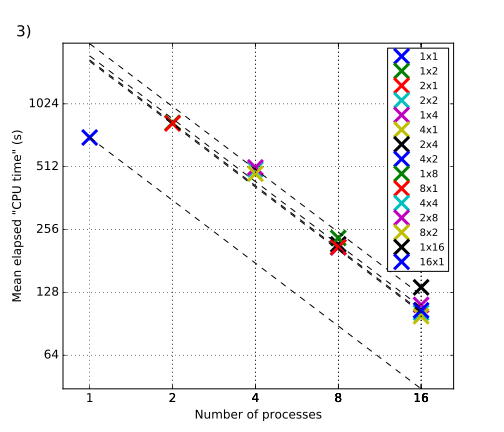
\includegraphics[width=0.5\textwidth]{met_c44xlarge.pdf}
	\caption{Time (in seconds) spent per process for the ROMS "medium" benchmark test (benchmark2.in), as function of the number of processes. The inset shows the tiling. Axes are logarithmic with base 2, dashed lines show slopes of "ideal" scaling functions with varying offset. Computations are performed on a c4.4xlarge instance, which has 16 vCPUs per (virtual) node.}
	\label{fig:met_c44xlarge}
\end{figure}

Fig. \ref{fig:met_c48xlarge} shows that \verb|benchmark3| has an execution time of roughly $230\,\rm s$ on 32-cores of a \verb|c4_8xlarge| instance using the GFortran compiler. The number of time steps integrated in  \verb|benchmark3| is 200, i.e. on time step is processed every $1.15\,\rm s $. Note that we use only 32 vCPUs of the c4.8xlarge to avoid potential problems with some Linux operating systems which have a vCPU limit of 32 \citep{web:ec2_c4}. 
Fig. \ref{fig:met_c48xlarge} shows the overhead induced by distributing the computation amongst various nodes. The networking configuration used in the experiment was the default configuration provided by \verb|CfnCluster|. In particular, we \emph{did not} verify whether the modifications described by \cite{web:cyclempi} \citep[see also][]{web:ibmMpiTrick} have been applied before the experiment was conducted. We hypothesize that any improvements gained by optimizing the infrastructure beyond the configuration provided by \verb|CfnCluster| will likely not decrease execution time by an order of magnitude. We assume that if this was the case, such an optimization would be adopted by \verb|CfnCluster|, or at least be described in their documentation.

\begin{figure}[H]
	\centering
	\includegraphics[width=0.5\textwidth]{met_c48xlarge.pdf}
	\caption{Time (in seconds) spent per process for the ROMS "large" benchmark test (benchmark3.in), as function of the number of processes.  Axes are logarithmic with base 2. Computations are performed on c4.8xlarge instances of AWS, which have 36 vCPUs per node.}
	\label{fig:met_c48xlarge}
\end{figure}

\subsection{Computational and monetary costs of a realistic study}

The preliminary test above allow a rough estimate of the computational and monetary costs involved in a realistic study. By monetary cost we mean the financial cost of renting AWS' hardware to conduct a study of a given computational cost. As an example we consider \cite{kumar2015midshelf}, who validate the midshelf and surfzone circulation generated by a numerical model against observations.  They use a coupled ROMS-SWAN model and compare it to observations from the 2006 Huntington Beach (San Pedro Bay, California, U.S.A.) experiment. We assume that such studies, which investigate the transport processes directly adjacent to the coast, are particularly important for commercial applications. Whether or not it is actually \emph{technically feasible} to conduct such a highly complex state-of-the-art simulation on AWS' cloud infrastructure, is not shown here. Instead, the objective here is to gain a (very rough) order-of-magnitude estimate of the involved cost, \emph{assuming} technical feasibility. 

\subsubsection{Components of the numerical experiment}

The numerical experiment of \cite{kumar2015midshelf} consists of the following components:

\begin{itemize}
	\item Wind forcing
	\item Wave forcing
	\item Tide forcing
	\item Buoyancy forcing
\end{itemize}

which are coupled by the open-source Coupled Ocean-Atmosphere-Wave-Sediment (COAWST) Transport model \citep{warner2008using,web:coawst}, which couples an atmospheric (Weather Research and Forecasting model, WRF), wave (SWAN), three-dimensional circulation and stratification (ROMS) and sediment transport models. COAWST is integrated by the Model Coupling Toolkit (MCT, \citealt{web:mct}) to exchange data fields between the models. They use the following nested grids:

\begin{itemize}
	\item U.S. West Coast and eastern Pacific (L0):  $\Delta=5\,\rm km$, area $4000\times3000\,\rm km^2$ ($800\times600\times40$ grid points)
	\item Southern California Bight (L1):  $\Delta=1\,\rm km$, area $800\times700\,\rm km^2$ ($800\times700\times40$ grid points)
	\item Interior bight region (L2): $\Delta=250\,\rm m$, area $500\times300\,\rm km^2$ ($2000\times1200\times40$ grid points)
	\item San Pedro Bay (L3): $\Delta=75\,\rm m$, area $80\times70\,\rm km^2$ ($1067\times934\times32$ grid points)
	\item Huntington Beach, Newport Beach (shelf break to inner shelf and surfzone): $\Delta=50\,\rm m$, area $15\times30\,\rm km^2$ ($214\times428\times20$ grid points)
	\item Huntington Beach (mid-shelf to surfzone): $\Delta=10\,\rm m$, area $6\times6\,\rm km^2$ ($600\times600\times20$ grid points)
\end{itemize}

 As boundary conditions (forcing fields) they use\footnote{\cite{kumar2015midshelf} provide an overview of their model set up, but understandably don't provide full detail. Our presentation may be inaccurate.}

\begin{itemize}
	\item Lateral forcing: The parent grid L0 is forced with a combination of lateral boundary conditions from an assimilated global oceanic dataset \citep{carton2008reanalysis}. Freshwater flux from river runoff is included. In addition, barotropic tidal elevation and velocities are projected onto the boundaries of L1.
	
	\item Surface forcing (wind-stress, heat, radiative and freshwater) is provided by a doubly nested WRF model with $\Delta=18\,\rm km$ (for L0) and $\Delta=6\,\rm km$ (for L1, L2, L3), embedded within the NCEP North American Regional Reanalysis. Surface temperature and salinity are relaxed to monthly averages from \cite{carton2008reanalysis}.
	
\end{itemize}

The L0-L5 domains are one-way nested, i.e. L0-L4 each provide boundary condition data for their respective child grid. Daily L0 solutions are used as a lateral boundary condition for L1. L1 (L2) solutions are used as L2 (L3) lateral boundary conditions every $2\,\rm h$. Note again that L1's boundary condition includes barotropic tidal elevation and velocities in addition to information provided by its parent.

The model is spun up for $15\,\rm yr$ with climatological surface forcing.


For time-stepping the shelf grids, \cite{kumar2015midshelf} state that

\begin{itemize}
	\item L4 and L5 are integrated for 92 days with a baroclininc time step of $8\,\rm s$ and $4\,\rm s$, respectively.
	\item wave action density in SWAN evolves with a time step of $120\,\rm s$ and $60\,\rm s$, respectively. Exchange of information between the circulation and wave models occurres every $360\,\rm s$.
\end{itemize}


\subsubsection{Computational cost}

\cite{kumar2015midshelf} do not report the time step used in their L0-L3 models. Assuming an ocean depth of $H=2000\,\rm m$, the barotropic time step $\Delta t_{bt}$ is constrained by the CFL condition to roughly $\mathcal{O}(10\,\rm s)$ for L0 and L1, and $\mathcal{O}(1\,\rm s)$ for L2 and L3, according to the simplified formula (which does not hold strictly in this practical application)

\begin{equation}\label{eq:cfl}
\Delta t_{bt}\leq\Delta x/c \qquad c=\sqrt{gH},
\end{equation}

where $\Delta t_{bt}$ ($\Delta x$) is the barotropic time step (lateral grid spacing), and $g$ is standard gravity (Tab. \ref{tab:timesteps}). 

\begin {table}[H]
\begin{center}
	\begin{tabular}{ l | r | r | r| r }
		           $\Delta x$     & $5\,\rm km$ & $1\,\rm km$ & $250\,\rm m$ & $75\,\rm m$\\
		 $\Delta t_{bt}$       &  $36\,\rm s$ & $7\,\rm s$   &$1.8\,\rm s$       &  $0.5\,\rm s$\\
		 $\Delta t$       &  $535\,\rm s$ & $107\,\rm s$   &$27\,\rm s$       &  $8\,\rm s$ \\
		 $N (10^6)$                  &  $0.9$ & $4.4$   &$18$       &  $59$
	\end{tabular}

\end{center}\caption{Barotropic ($\Delta t_{bt}$) and baroclinic ($\Delta t$) time steps for various grid resolutions ($\Delta x$), assuming validity of Eq. \eqref{eq:cfl}, a depth of $H=2000\,\rm m$,  and  $\Delta t/\Delta t_{bt}=15$. $N$ is the number of timesteps required for a $15\,\rm y$ model simulation (divided by $10^6$), the last column lists the total run time of a $15\,\rm y$ simulation.}\label{tab:timesteps}
\end{table}

Assuming that the baroclinic time step $\Delta t$ is a factor of 10-20 longer than the barotropic time step, this yields $\Delta t=\mathcal{O}(100\,\rm s)$ (L0, L1) and $\Delta t= \mathcal{O}(10\,\rm s)$ (L2, L3), respectively. For a $15\,\rm yr$ simulation, $N=\mathcal{O}(10^6)$ ($N=\mathcal{O}(10^7)$) baroclinic time steps are required for L0, L1 (L2, L3). Clearly, these estimates are very rough. For example, to account for the shallower depth of the L2 and L3 grids,  one may assume a depth decrease by a factor of 10, and accordingly increase $\Delta t_{bt}$ by a factor of 3 for L2 and L3. 

So far, no results are available measuring execution time for grids of similar size as L0-L3. The closest match is \verb|benchmark3|, with a grid size of $2048$ x $256$ x $30$ data points, which is roughly 80\% (15\%) of the number of spatial data points in L0 (L2). Note that it is always possible to assume identical physical dimensions of the grid spacing (including the temporal lattice) between \verb|benchmark3| and L0-L3, since the benchmarking results are independent on physical dimensions (but depend only on the amount of data points).

Our results showed that in \verb|benchmark3|, the processing time for one time step is about $1.15\,\rm s$ seconds using 32 cores of a single \verb|c4_8xlarge| instance. It follows that a $15\,\rm yr$ spin up time for \verb|benchmark3|  (assumed to consist of $10^6$-$10^7$ baroclinic time steps of lenghts displayed in Tab. \ref{tab:timesteps}) takes a minimum of $\mathcal{O}(10\,\rm d)$ to complete.

\subsubsection{Monetary cost}

The instance type \verb|c4_8xlarge| is currently (2017/01/12) priced at \textdollar 1.591 (2.085) per Hour for on-demand use in US East (Asia Pacific, Sydney) region, resulting in a total of roughly $\mathcal{O}(\text{USD } 500)$ for a 10 day lease.



\subsection{Conclusion}

Given that high-resolution, state-of-the-art regional and coastal numerical studies such as  \cite{kumar2015midshelf} are conducted on multiple different large grids (some of which require an extensive spin-up phase) we estimate that the total monetary cost of cloud-computing infrastructure will typically be on the order of $\mathcal{O}(\text{USD } 10,000)$ to $\mathcal{O}(\text{USD } 100,000)$. Note that this estimate refers to the final experiment(s) whose results are published. Importantly, it \emph{does not} include the testing phase, which may well increase the total cost of the study by a factor of 10 or more. 

\subsection{TODO}

Compare it to cost of acquiring and operating computers.

	
\bibliography{main.bib}
\bibliographystyle{model2-names}

\end{document}

 
